\chapter{畫圖測試}

\begin{minipage}[htpb]{80mm}
	%\begin{center}
    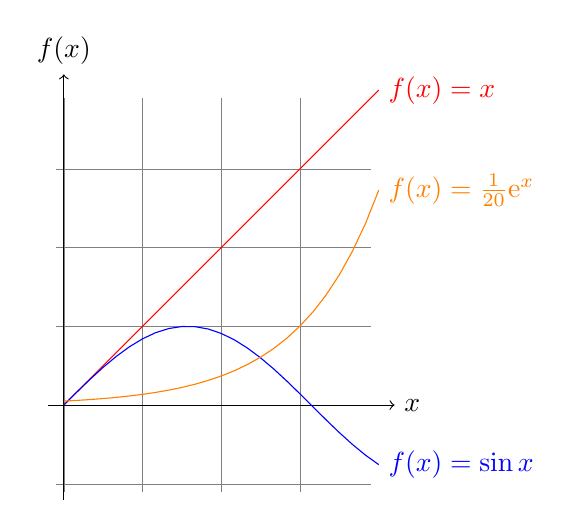
\begin{tikzpicture}[domain=0:4]
		  \draw[very thin,color=gray] (-0.1,-1.1) grid (3.9,3.9);
  		\draw[->] (-0.2,0) -- (4.2,0) node[right] {$x$};
		  \draw[->] (0,-1.2) -- (0,4.2) node[above] {$f(x)$};
		  \draw[color=red]    plot (\x,\x)             node[right] {$f(x) =x$};
  % \x r 表示弧度
		  \draw[color=blue]   plot (\x,{sin(\x r)})    node[right] {$f(x) = \sin x$};
		  \draw[color=orange] plot (\x,{0.05*exp(\x)}) node[right] {$f(x) = \frac{1}{20} \mathrm e^x$};
		\end{tikzpicture}
	%\end{center}
\end{minipage}



\begin{minipage}[htpb][80mm][t]{80mm}
	%\begin{center}
		\vspace*{60mm}
    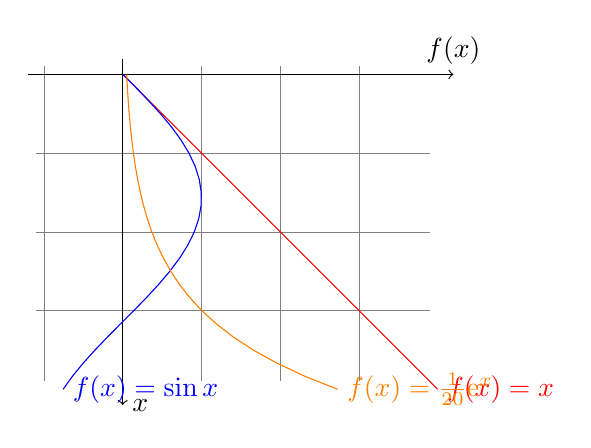
\begin{tikzpicture}[domain=0:4,scale=1,rotate=270]
		  \draw[very thin,color=gray] (-0.1,-1.1) grid (3.9,3.9);
  		\draw[->] (-0.2,0) -- (4.2,0) node[right] {$x$};
		  \draw[->] (0,-1.2) -- (0,4.2) node[above] {$f(x)$};
		  \draw[color=red]    plot (\x,\x)             node[right] {$f(x) =x$};
  % \x r 表示弧度
		  \draw[color=blue]   plot (\x,{sin(\x r)})    node[right] {$f(x) = \sin x$};
		  \draw[color=orange] plot (\x,{0.05*exp(\x)}) node[right] {$f(x) = \frac{1}{20} \mathrm e^x$};
		\end{tikzpicture}
	%\end{center}
\end{minipage}

% \chapter{公式測試}

\vskip 20 mm
\begin{minipage}[htpb]{80mm}
		\vspace*{45mm}
	%\begin{center}
			{\normalsize With normalsize 10 pt in class (truely 9.13\,pt in real dimen):
				\[ \sampleEq \]\par}

			{\Large With Large 14 pt in class (truely 12.782\,pt in real dimen):
				\[ \sampleEq \]\par}

			{\footnotesize With footnotesize 8 pt in class (truely 7.304\,pt in real dimen):
				\[ \sampleEq \]\par}
	%\end{center}
\end{minipage}

\clearpage
\begin{minipage}[htpb]{120mm}
		\vspace*{10mm}
	%\begin{center}
			{\normalsize 
				\[ \sampleEq \]\par}

			{\Large 
				\[ \sampleEq \]\par}

			{\footnotesize
				\[ \sampleEq \]\par}
	%\end{center}
\end{minipage}